\documentclass[12pt]{article}
\usepackage{geometry} % see geometry.pdf on how to lay out the page. There's lots.
\usepackage{natbib}
\usepackage{graphicx}
\usepackage{url}
\usepackage{color}
\geometry{a4paper} 
\usepackage{chngcntr}
\counterwithin{table}{section}

%%%%%%%%%%%%%%%%
%%%%%%%%%%%%%%


\title{Double blind reviewing at EvoLang 11\\reveals gender bias}
%\author{Se\'{a}n G. Roberts* \\
%Language and Cognition Department, \\Max Planck Institute for Psycholinguistics, \\Nijmegen, Netherlands  \\\\
%Tessa Verhoef* \\
%Center for Research in Language,\\University of California,\\San Diego, San Diego, USA\\
%\small *These authors contributed equally}
\date{} % delete this line to display the current date

%%% BEGIN DOCUMENT
\begin{document}
\maketitle
%%%%%%%%%%%%%%
%%%%%%%%%
 %
%
 %


\section*{Abstract}
The impact of introducing double blind reviewing in the most recent Evolution of Language conference is assessed.  The ranking of papers is compared between EvoLang 11 (double blind review) and EvoLang 9 and 10 (single blind review).  Main effects were found for first author gender by conference.  The results mirror some findings in the literature on the effects of double blind review, suggesting that it helps reduce a bias against female authors.

\section{Introduction}

Every two years since 1996, The Evolution of Language (EvoLang) conference has been a major international event for research on the origins and evolution of language.  The 11th EvoLang (\citealp{roberts2016evolution} (see \url{http://evolang.org/neworleans/}) introduced double blind review (DBR), as compared to single blind review used in all previous conferences. This paper assesses whether there are any detectable effects of this change, focussing on gender and whether papers are authored by students or more established researchers.

There is a growing body of literature on biases within academia. These include the Matilda effect, a bias against women in male dominated fields \citep{knobloch2013matilda}, and the Matthew effect, a bias favouring well-established academics \citep{merton1968matthew}.  The Matilda effect has been found in various areas of academia (see \citealp{EU2012meta,Science_WomenInScience}). 

Previous findings vary, but many show that female authored papers are accepted more often or rated higher under DBR \citep{snodgrass2006single,budden2008double}.  The trend is similar in other areas, for example a recent (unpublished) study found that female authored code had higher acceptance rates in collaborative software projects when their gender was not identifiable \citep{terrell2016gender}.  

However, some studies found no difference in gender balance as a result of DBR \citep{primack2009gender,whittaker2008journal}.  \cite{webb2008does} and \cite{engqvist2008double} argue that the increase in ratings of female authored papers is partly caused simply by an increasing number of females in the pool of submitters or a general reduction in bias over time, rather than an effect of review type.  There are also other potential effects which are not explored here, for example the prestige of an institution \citep{blank1991effects}. 

Arguably, the field of language evolution is a male-type topic, or at least dominated by male authors.  For example, in the `Language Evolution and Computation bibliography'\footnote{maintained until 2013, \url{http://www.langev.com/author}}, only 8 out of the top 100 most cited authors are female.  Also, only 9 out of 77 invited plenary speakers to the EvoLang conferences before 2016 were female (with the most recent conference being a welcome improvement of 5 females out of 9 invited speakers).  Therefore this field could be susceptible to the Matilda effect.  The effect of author prestige is harder to predict: the field is small enough that researchers know each other, but young enough that there are few well-established researchers whose primary topic is language evolution. 

\section{Analysis}

\subsection{Data}

Data was available for 176 submissions from EvoLang 9 \citep{scott2012evolution}, 191 submissions from EvoLang 10 \citep{cartmill2014evolution} and 196 submissions from EvoLang 11 \citep{roberts2016evolution}.  For each submission, the mean reviewers' score and ranking within each conference was calculated, and scaled (0 = worst, 1 = best, average rank used for ties).  Authors specified their student status.  Gender of the first author was coded (by SR) using a binary male/female categorisation based on a subjective assessment of the authors' performed gender on their academic profile.  Throughout this paper, only the identity of the first author is considered.  Table \ref{tab:count} shows the number of submissions by gender and student status for each conference. 

\begin{table}[htbp]
\begin{center}
\begin{tabular}{l | l l | l l}
	   & Non-Student & & Student & \\
         &    Female & Male & Female & Male\\
         \hline
  EvoLang 9  &34 & 85 & 18 & 45 \\
  EvoLang 10& 55& 94 &  12 & 30\\
  EvoLang 11& 40 &78   &32 & 45\\
\end{tabular}
\end{center}
\label{tab:count}
\caption{Counts of submissions in the data by gender and student status.}
\end{table}%

Analyses are complicated by differences in the proportion of students between conferences and multiple papers being written by the same authors.  Therefore, the \emph{paired change in ranking} was analysed, which keeps the identity of the first author constant.  Authors were identified who submitted a paper to multiple conferences, and an anonymous identification number for each of these authors was added.  73 authors (29 female, 24 student) were identified who applied to both EvoLang 10 and EvoLang 11 (25\% of unique authors, 165 submissions, authors could submit a maximum of 2 papers to each conference, data on EvoLang 9 was discarded because only 30 authors had submitted to the last 3 conferences, only 9 of which were female).  For each author, the change in ranking between their best ranked paper in EvoLang 10 and EvoLang 11 was calculated. Student status was determined by authors' reported student status in Evolang 10.  For full data and analysis, see the supporting information or \url{https://github.com/seannyD/EvoLangDoubleBlindData}.

\subsection{Results}

Overall, reviewers gave papers in later conferences higher raw scores (ANOVA F = 16.25, df = 2, p $<$ 0.001), so the main analyses were carried out using the scaled ranking of papers.  Figure \ref{fig:gen} and figure \ref{fig:stu} show the distribution of rankings by gender and student status for each conference.  

\begin{figure}[htbp]
\begin{center}
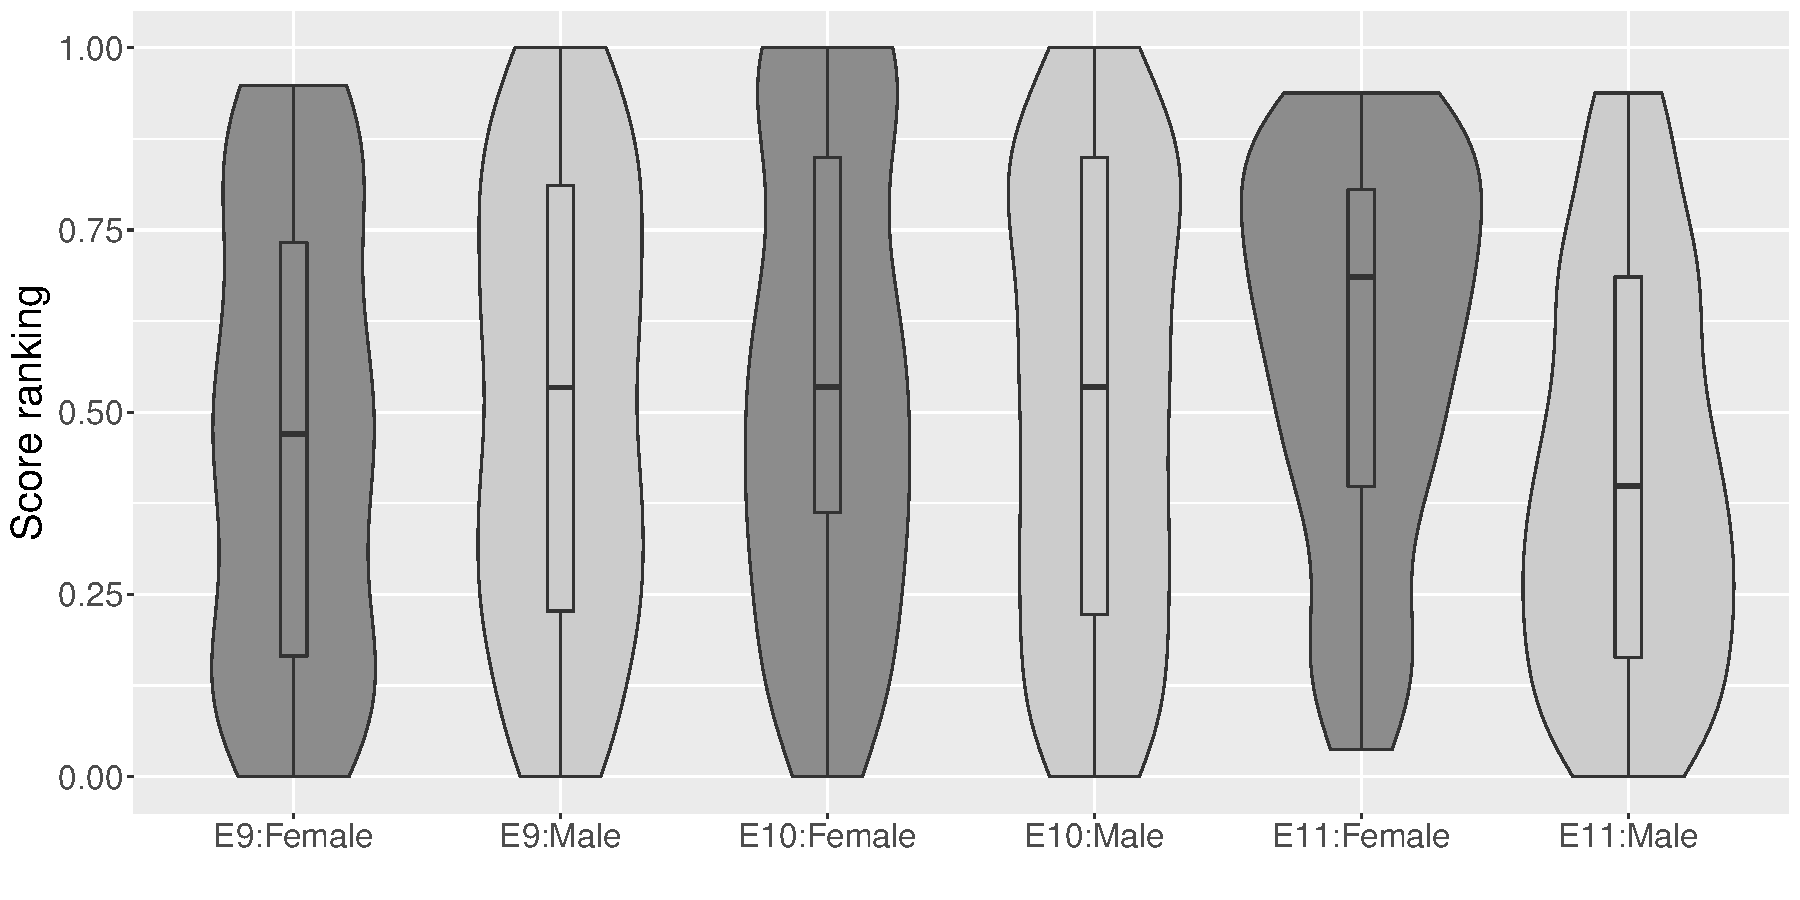
\includegraphics[width=130mm]{../Results_Gender_3conf.pdf}

\caption{Differences in ranking by gender of first author.}
\label{fig:gen}
\end{center}
\end{figure}


\begin{figure}[htbp]
\begin{center}
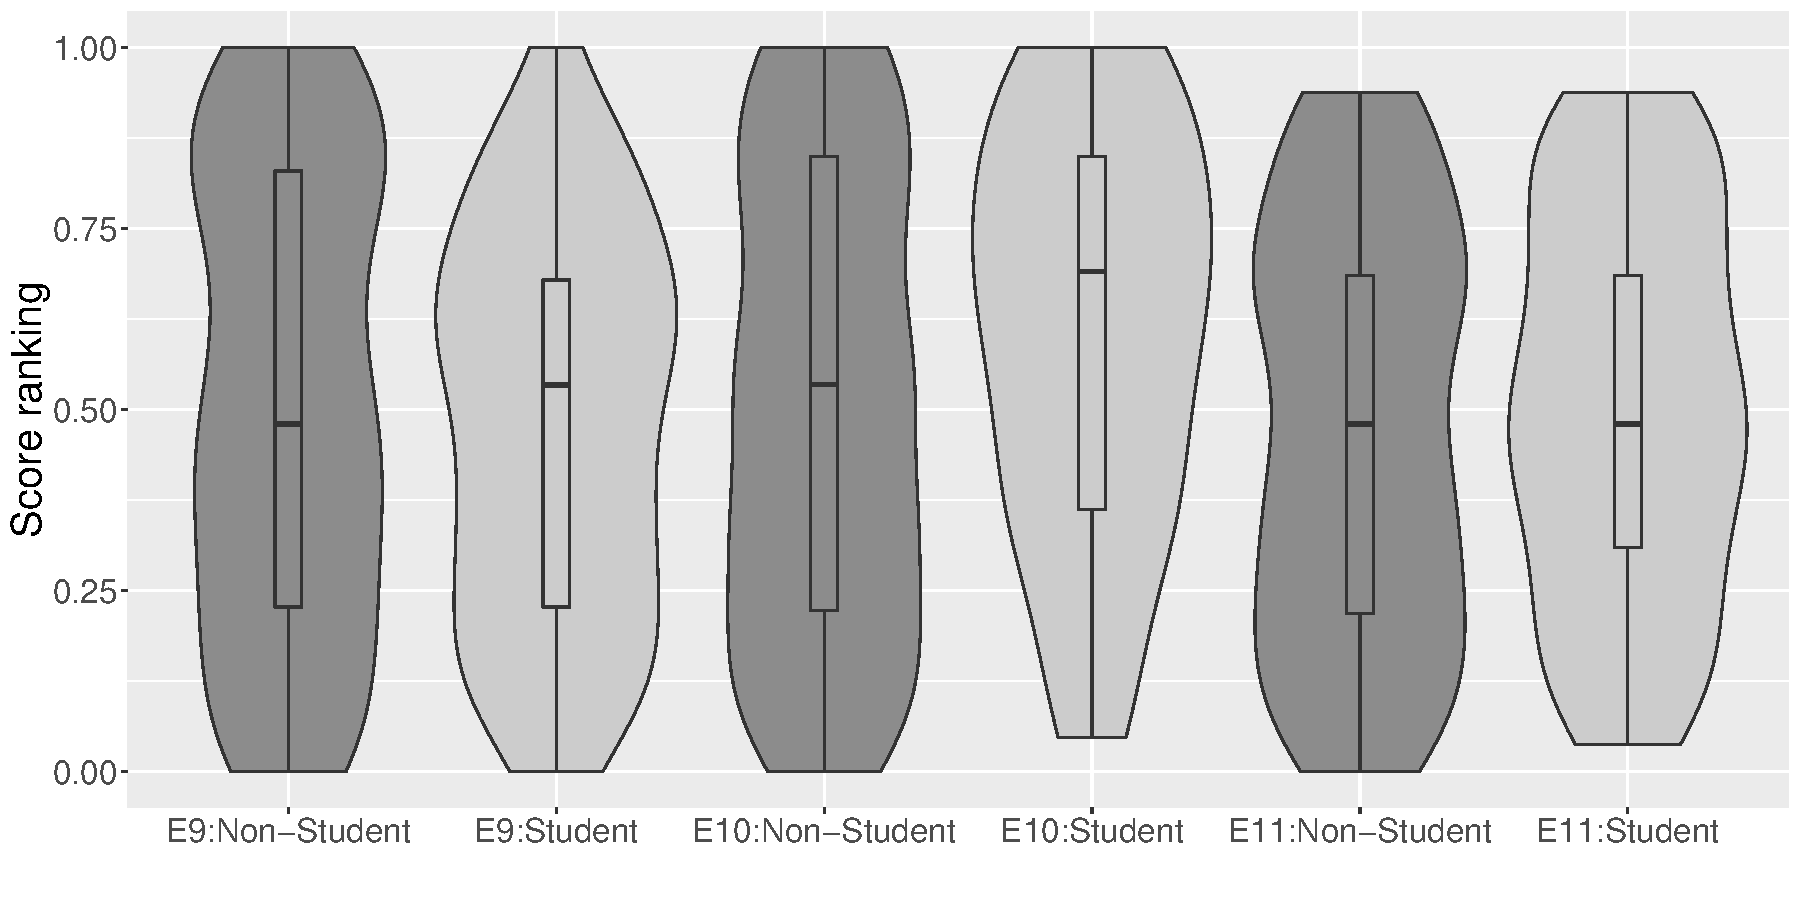
\includegraphics[width=130mm]{../Results_Student_3conf.pdf}

\caption{Differences in ranking by student status of first author.}
\label{fig:stu}
\end{center}
\end{figure}


We performed a three-way independent samples ANOVA on paper ranking by gender, student status, conference, and all interactions between the independent variables.  There was a significant main effect of first author gender (F(1) = 5.65, p = 0.018).  There was also a significant interaction between first author gender and conference (F(2) = 5.81, p = 0.003).  No other factors were significant. 

Post-hoc t-tests showed that there was little difference in ranks for papers with male or female first authors for EvoLang 9 (difference in means = 0.04, t = -0.87, p = 0.386) or EvoLang 10 (difference in means = -0.04, t = 0.75, p = 0.454), but there was a difference in EvoLang 11 (difference in means = -0.17, t = 4.4, p $<$ 0.0001).  In other words, female first-authored papers ranked higher in the conference with DBR.

Regarding the data on paired change in ranking, the average change over the two conferences was a drop of about 7\% (a large number of first-time submitters in EvoLang 11 received good reviews).  A linear regression was used to predict the change in author ranking over the two conferences by gender and student status.  There was a significant effect of gender (female authored papers ranked higher by about 4\% over the two years on average while male author ranking declined by about 19\% on average, t = -2.19, p = 0.03), and no effect of student status (t = -1.58, p = 0.12).   There was also a significant interaction between gender and student status (t = 2.19, p = 0.03).  The ranking of student papers declined on average by 20\%, but in contrast male students improved by 14\%. Figure \ref{fig:imp} shows the paired change in ranking by gender and student status.

\begin{figure}[htbp]
\begin{center}
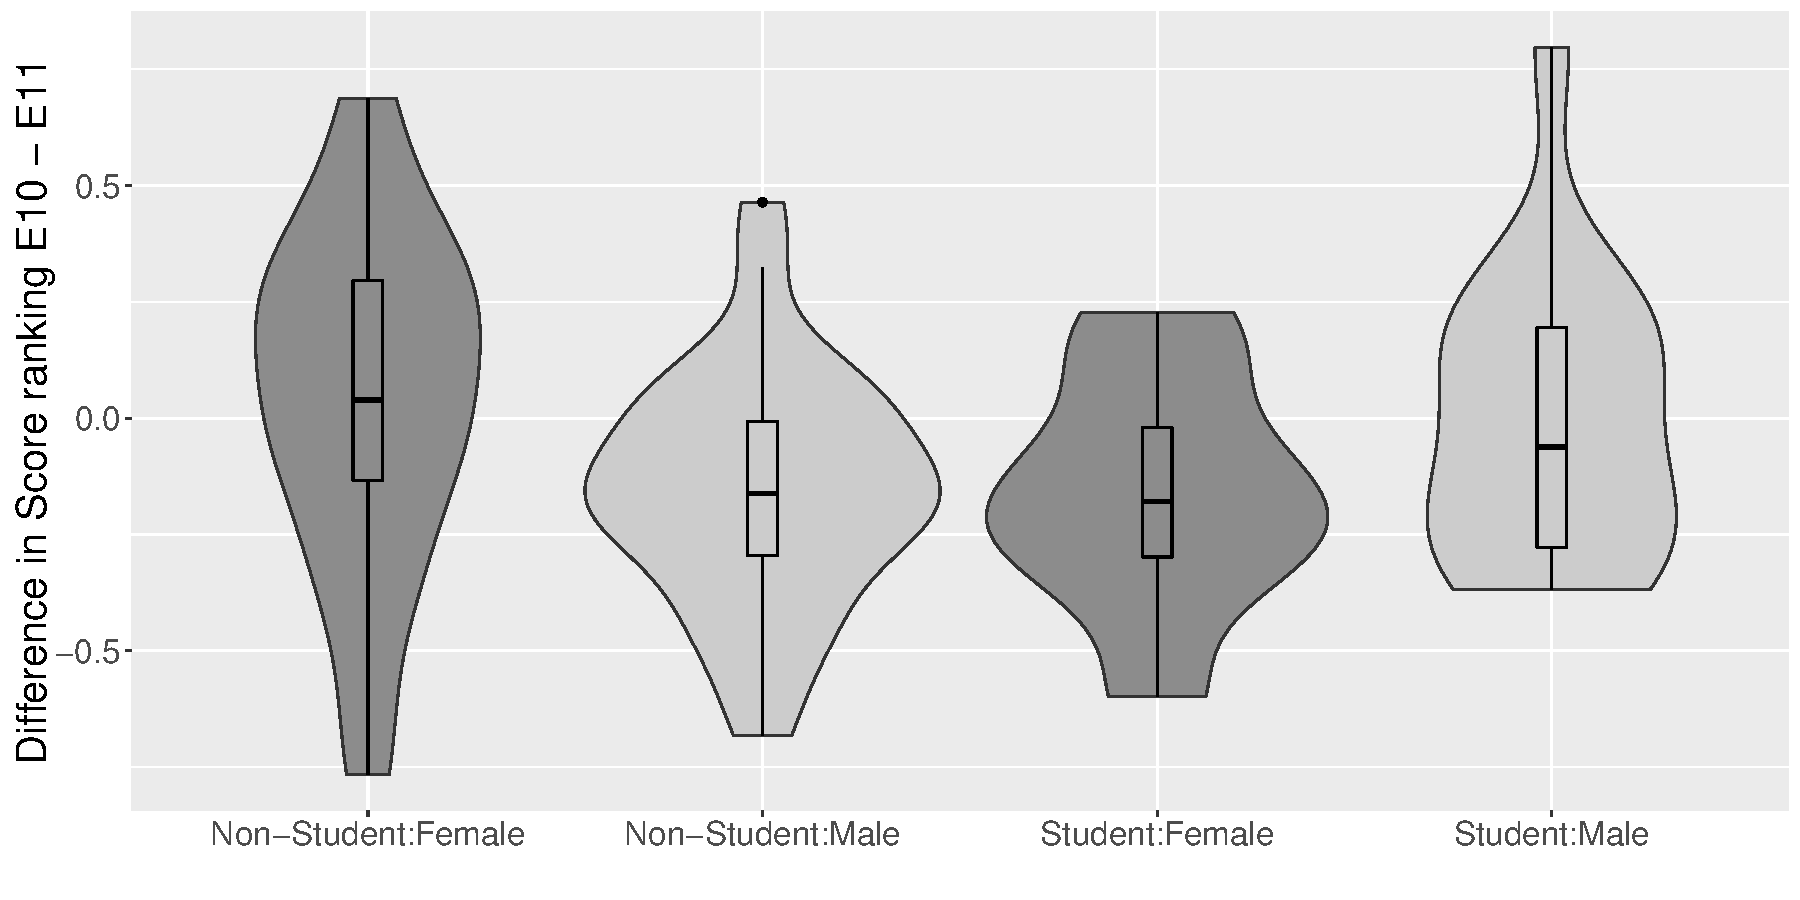
\includegraphics[width=130mm]{../Improvement.pdf}
\caption{Paired change in ranking by identity of the first author.  A positive value indicates that the author's best paper is ranked higher in E11 than E10.}
\label{fig:imp}
\end{center}
\end{figure}

The supplementary materials include an attempt to analyse whether the bias differs by the gender type of the research topic, but found no significant results.

\section{Discussion}

This study explored the differences between review scores in three EvoLang conferences, including two single-blind conferences and the most recent double-blind conference.  The first finding is that there are proportionality fewer papers submitted by female first authors overall, which itself is an indication of a bias.

Regarding student status, in general student papers were rated as better than non-student papers, which was less prominent in EvoLang 11.  This might be explained by authors being more lenient towards student papers (or, conversely, more critical of minor problems by established authors), and this effect is then minimised under DBR.  That is, there was no evidence for the Matthew effect in the overall data.

Regarding gender, in the conferences with single blind review there was little difference in ranking between genders, but female first-authored papers were ranked higher under DBR.  When looking at papers by the same authors in both conferences, female authored papers move up in ranking while male authored papers are ranked lower, though this happened mainly for non-students.

This fits with some previous findings in the literature showing a reduction in bias against female authors in DBR.  It is interesting to note that, in this data, the bias is only revealed under DBR.  That is, equality in ratings between genders is not a guarantee of bias-free review.  The gender coding of the field or sub-topic may be a relevant consideration, but no evidence could be found for an effect in our data (see supplementary materials).  

There are many possible explanations for the effect of gender. One is a general bias against female authors, prompting them to compensate by putting more effort into their submissions, and this effort is recognised once the gender bias is removed under DBR.  However, that would not explain the interaction between gender and student status discovered in the paired data.  Since the author's name does not directly reveal their student status, any effect should be due to whether the person is known in the field or not.  So the second result might be explained by a combination of gender bias and prestige bias (the ratings of well-known males are most inflated by the bias, and so decline more under DBR).  

It is possible, as papers cited above argue, that the improvement scores for female authored papers could just be driven by a larger sample of female authors in later conferences.  However, that would not explain the differences we find when looking at the paired data.  Another possibility is that the data do show a bias, but reflect a general improvement in attitudes towards gender over time, rather than an effect of DBR.  The fact that the distribution of rankings changed very little between Evolang 9 and 10 and was strikingly different in Evolang 11 may suggest that the change in review type played a role, but more data is needed to fully test which hypothesis has more support. 

Future studies could consider the issues above, drawing on data from future EvoLang conferences while also gathering data on other aspects of equality, such as racial diversity.  For other suggestions of practical steps, see \cite{martin2014ten}.  It is important to note that while DBR might help reduce the effects of reviewer biases, it does not solve the problem of biases themselves.  However, there may be a positive indirect effect if double blind reviewing leads to an increased female participation in conferences.  DBR requires more careful organisation of the reviewing process, but appears to have few negative effects.  Therefore, given the possible positive effect of reduced bias and a greater emphasis on merit, it is the recommendation of this paper that double blind reviewing continue to be used at future EvoLang conferences.


%\section*{Acknowledgements}
%SR is supported by the Interactional Foundations of Language project and ERC Advanced Grant No. 269484 INTERACT to S. C. Levinson within the Language and Cognition Department at the Max Planck Institute for Psycholinguistics.  TV is supported by a Netherlands Organisation for Scientific Research (NWO) Rubicon grant. We would like to thank Julia Udden and Sonja Vernes for helpful comments.


%%%%%%%%%%
%%%%%%%


\bibliographystyle{apalike}
\bibliography{Biblography}


\end{document}

